% Padrão: false
\newif\ifprint
%\printtrue
%
\documentclass[a4paper,twocolumn,openright,article,12pt]{memoir}
\usepackage[portuguese]{babel}
\usepackage[utf8]{inputenc}
\usepackage{hyperref}
\usepackage{titlesec}
\usepackage[all]{hypcap}
\usepackage{geometry}
%\usepackage{arevtext,arevmath}
\usepackage{multirow}
\usepackage{tikz}
\usepackage{ctable}
%%%%%%%%%%%%%%%%%%%%%%%%%%%%%%%%%%%%%%%%

\renewcommand{\familydefault}{\sfdefault}
%\title{4\textordfeminine\ Conferência\\Latino Americana de\\Computação Científica e Python}
\titleformat{\chapter}[display]
{\bfseries\LARGE\sffamily}{\chaptertitlename}{10pt}{\LARGE}
\titlespacing*{\chapter}{0pt}{10pt}{10pt}
% \numberwithin{table}{chapter}

\begin{document}

\newgeometry{left=0cm, bottom=0cm, top=0cm, right=0cm}
\thispagestyle{empty}
\onecolumn
\ifprint
	\begin{center}
		\begin{tikzpicture}[remember picture, overlay]
    		\node[anchor=east] at (9,-5) {\fontsize{30}{30}\selectfont 4a. Conferência};
            \node[anchor=east] at (9,-6.3) {\fontsize{30}{30}\selectfont Latino Americana de};
            \node[anchor=east] at (9,-7.6) {\fontsize{30}{30}\selectfont Computação Científica e Python};
    		\draw[rectangle, fill] (-8,-3) -- (9,-3) -- (4,-3.1) -- (-3,-3.1);
            \draw[rectangle, fill] (-8,-9.6) -- (9,-9.6) -- (4,-9.7) -- (-3,-9.7);
    		\node at (current page.center) {\begin{minipage}{\textwidth}\centering \fontsize{20}{20}\selectfont Maio de 2016 \textendash\ Florianópolis \textendash\ SC\\\centering Brasil\end{minipage}};
		    \draw[rectangle, fill] (-10.8,-25.5) -- (10.75,-25.5) -- (10.75,-27.55) -- (-10.8,-27.55);
		    \node[color=white] at (-0.5,-26.6) {\fontsize{20}{30}\selectfont \textbf{conf.scipyla.org}};
		\end{tikzpicture}
	\end{center}
\else
	\begin{center}
          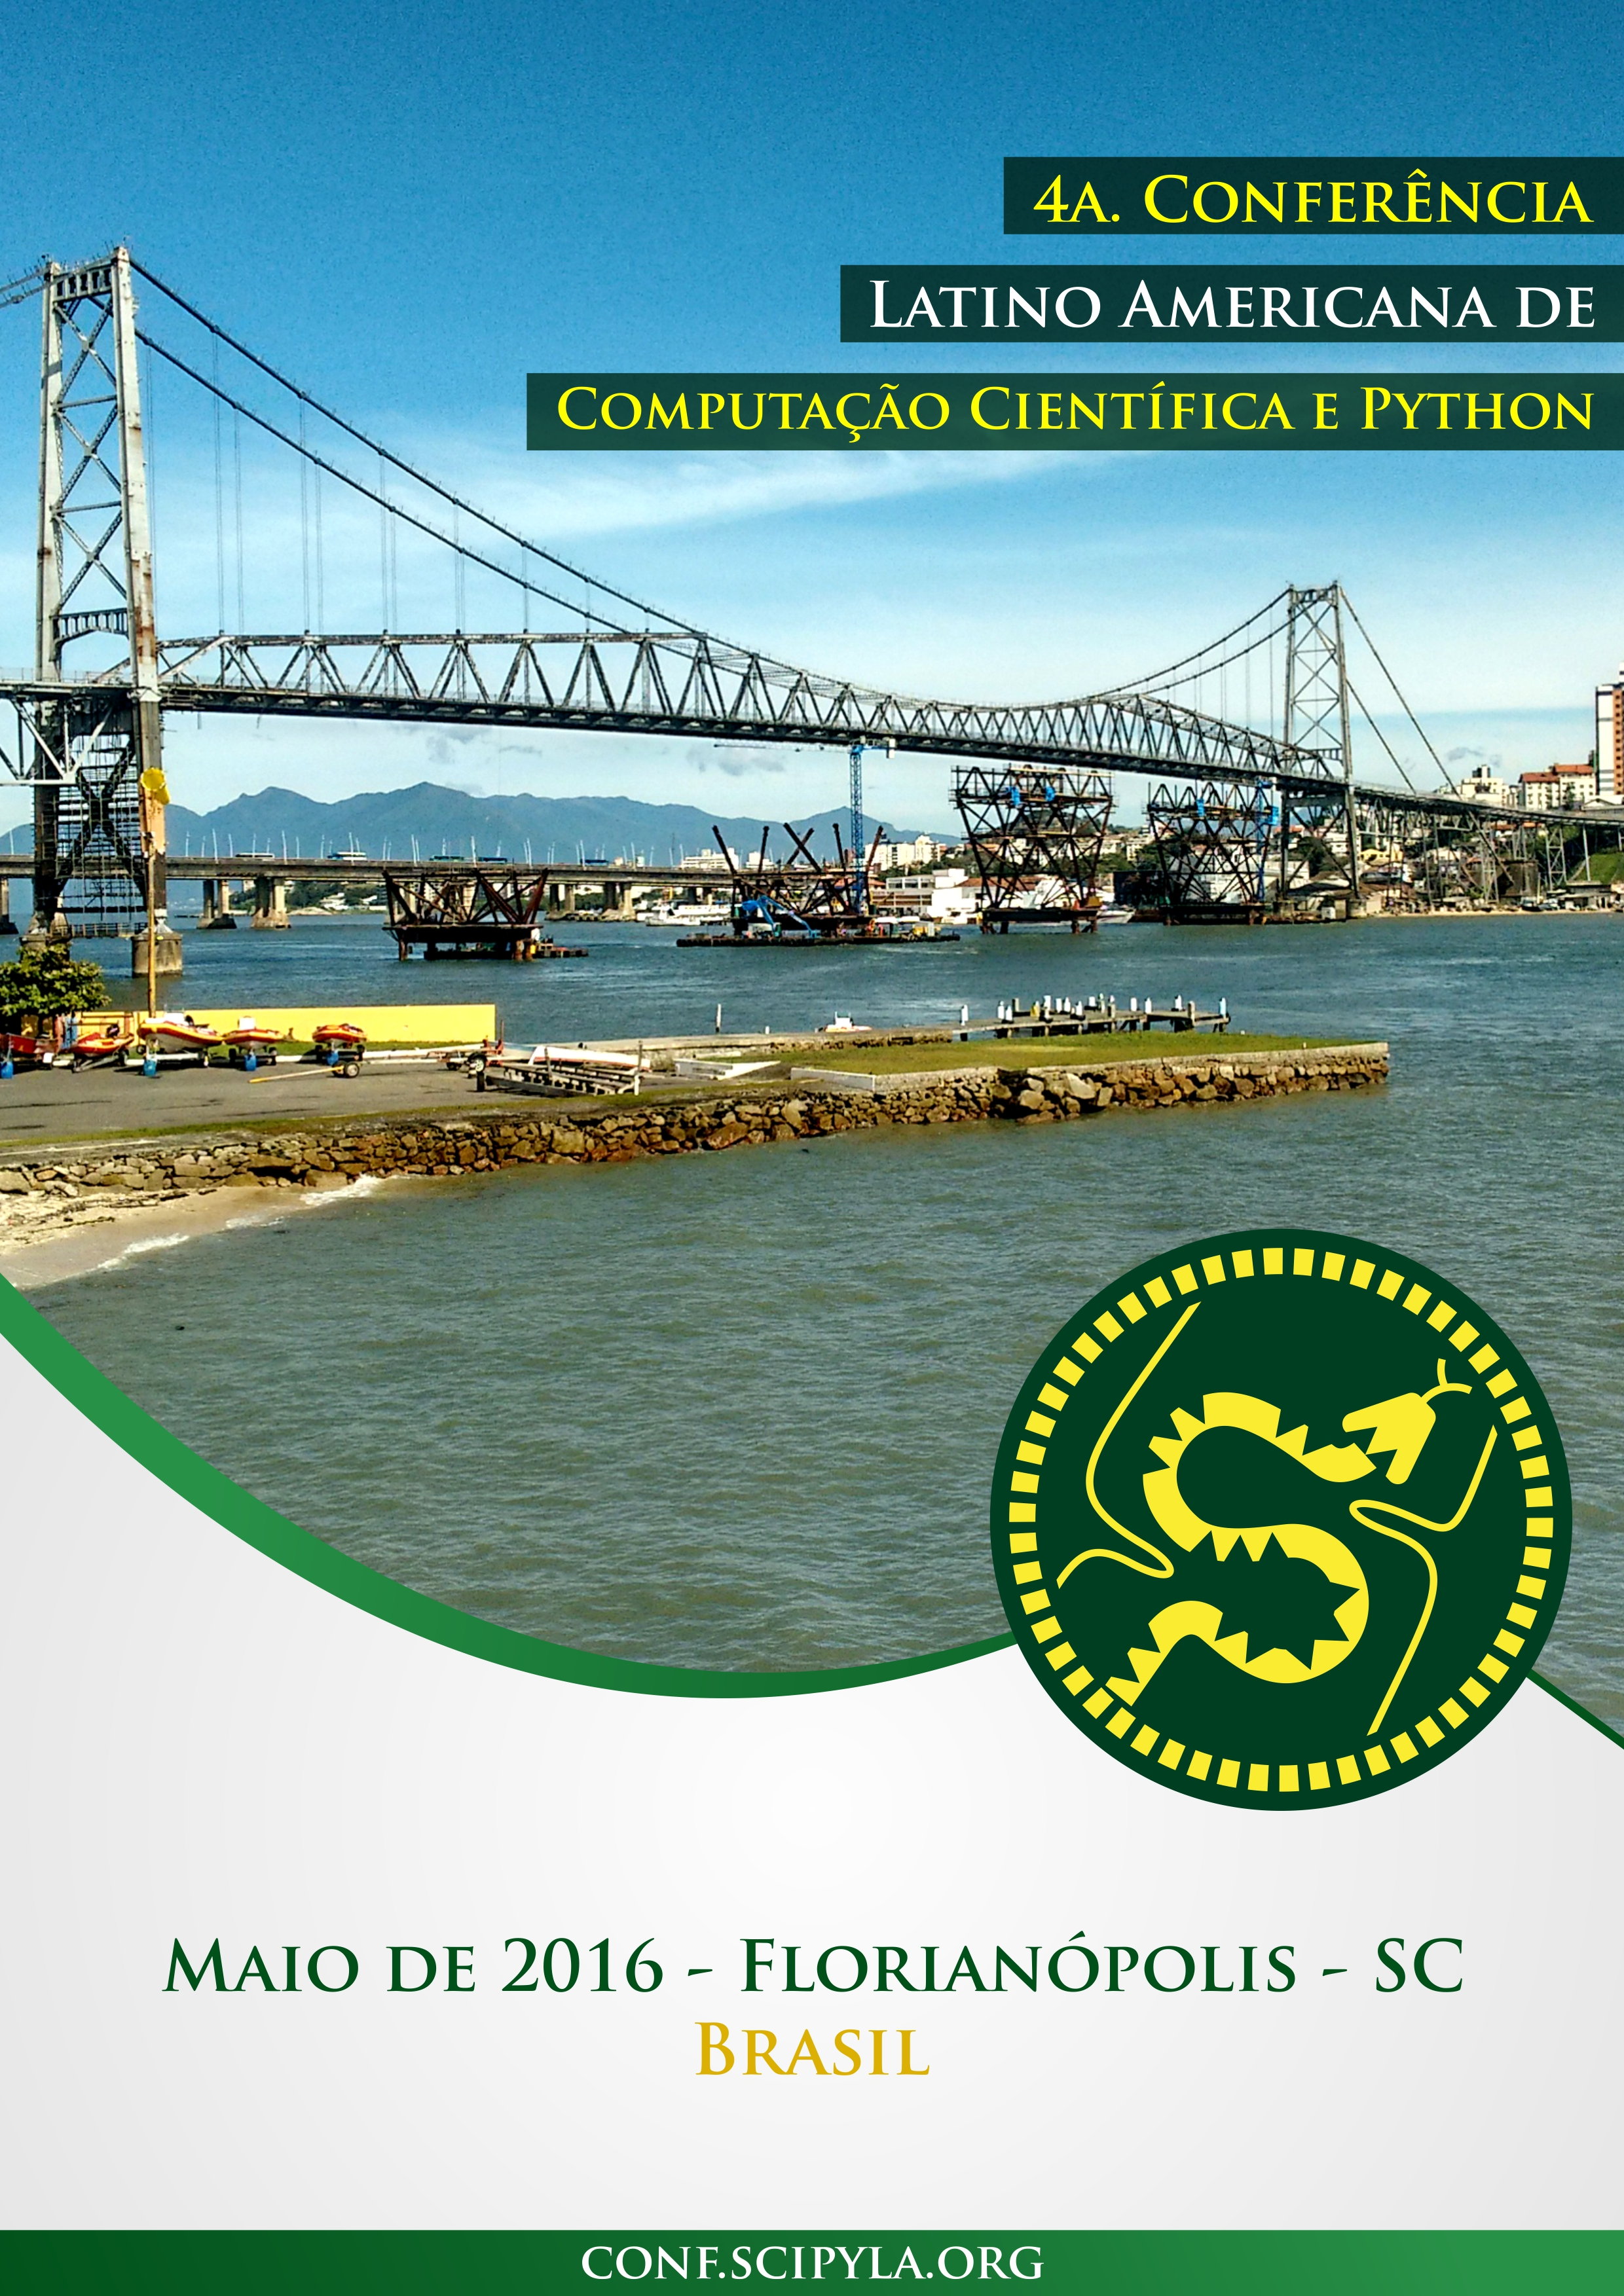
\includegraphics{../../media/img/capa.jpg}
	\end{center}
\fi
\twocolumn

\clearpage

\restoregeometry
\pagestyle{plain} % No headers, just page numbers
\setcounter{page}{2}
\tableofcontents*

\chapter*{Apresentação}
\addcontentsline{toc}{chapter}{Apresentação}

SciPy Latin America 2016, a quarta conferência anual de Computação Científica com Python, será realizada entre os dias 16 e 20 de maio de 2016, em Florianópolis / Brasil.

A conferência SciPy Latin America é focada em aplicações científicas e afins que
utilizam Python, seguindo o exemplo de outras conferências regionais de mesmo tema que ocorrem na Europa (EuroSciPy), Índia (SciPy India) e Estados Unidos (SciPy). Esse encontro sucede 3 outros encontros de mesma temática ocorridos na Argentina em 2013, 2014 e 2015.

O citado encontro consistirá de várias oficinas e palestras voltadas a pesquisadores, professores de diferentes níveis educacionais, estudantes, profissionais e empresários.

A comunidade SciPy é dedicada ao avanço da computação científica através de softwares \emph{open source} em Python para, mas não limitado a, Ciências Exatas, Biológicas, Humanas, e da Terra.

Tomando-se por base os encontros anteriores realizados na Argentina e Brasil, espera-se uma participação de aproximadamente 200 participantes provenientes das mais diferentes regiões. Na conferência palestrarão destacados pesquisadores de universidades Latinoamericanas e do mundo.

A organização da conferência oferece auxílio financeiro parcial para participantes,
palestrantes e membros do comitê organizador de forma que o evento seja inclusivo.
A verba para o auxílio financeiro, normalmente, é proveniente
de instituições públicas e privadas.

O êxito desta conferência é muito importante para a comunidade educacional, científica e industrial, e todos os demais influenciados por estas.

\ifprint
\else
	\begin{center}
          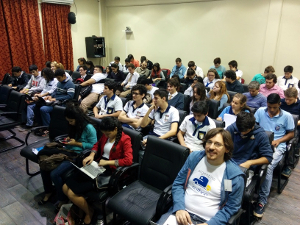
\includegraphics[width=6cm]{../../media/img/IMG_20150521_102157-small.jpg}
	\end{center}
\fi

\chapter*{Metodologia}
\addcontentsline{toc}{chapter}{Metodologia}

A conferência será voltada para a divulgação de ferramentas e/ou projetos realizados com Python no ambiente científico, acadêmico e industrial, e seus principais objetivos incluem:
\begin{itemize}
\item Dar oportunidade a divulgação da linguagem Python na comunidade científica Latinoamericana;
\item Divulgar e/ou revisitar ferramentas disponíveis aplicadas a problemas científicos ou outras de natureza similar;
\item Apresentar bibliotecas científicas desenvolvidas pela comunidade;
\item Combinar educação, engenharia e ciência através de Python;
\item Criar um marco apropriado para realização de encontros, fóruns de discussão, projetos educativos e de pesquisa relacionados a Python.
\end{itemize}

A organização e o desenvolvimento da conferência serão encaminhados por um comitê de docentes da Universidade Federal de Santa Catarina, entidades parceiras e membros da comunidade SciPy Latin América, localizados em diferentes países.

\ifprint
\else
	\begin{center}
          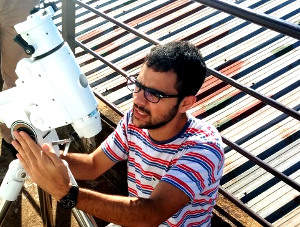
\includegraphics[width=6cm]{../../media/img/IMG_20150521_102919-small.jpg}
	\end{center}
\fi

\chapter*{Modalidades de apresentação}
\addcontentsline{toc}{chapter}{Modalidades de apresentação}

Haverá
%4
cinco
%
modalidades de apresentação de trabalhos:
\begin{itemize}
\item Palestras;
\item Pôsteres;
\item Tutoriais;
\item Palestras relâmpago;
\item Track Teen.
\end{itemize}

\section*{Palestras}

São as tradicionais palestras oferecidas aos dias principais da conferência. Possuem duração máxima de 30 minutos com 5 minutos para perguntas. Se você acredita
que possui um tema mas não sabe como escrever a proposta, contate nosso comitê
de atividades e iremos lhe ajudar nessa tarefa. Adoraremos ajudá-lo a submeter
uma ótima proposta.

\section*{Tutoriais}

Estamos procurando por tutoriais que possam ajudar a comunidade a crescer em qualquer nível. Nossa meta é ter tutoriais que possam avançar a computação científica com Python, melhorar a comunidade e moldar o futuro. Tutoriais possuem duração de 100-120 minutos, mas se você acredita que precisa de mais de um \emph{slot}, você pode dividir o conteúdo e submeter duas propostas que se complementam, mas que são independentes.

\section*{Pôsteres}

A sessão de pôsteres oferece uma apresentação mais interativa e direcionada ao público do que as palestras. A ideia é apresentar seu tópico no pôster e quando os participantes trocam de salas eles encontram seu trabalho, leem o que você escreveu e iniciam uma discussão sobre ele. Simples assim. Você pode fazer uma sessão de perguntas e respostas nos primeiros minutos da sessão com um grupo de 10 pessoas.

\section*{Palestras relâmpago}

Deseja dar uma palestra, mas não tem material suficiente para uma? Essas palestras são de, no máximo, 5 minutos em uma sequência de palestras similares no salão principal. Não é preciso preencher todo os tempo disponível. A inscrição dessa modalidade será realizada durante o evento até a última apresentação do dia.

\section*{Track Teen}

O Track Teen é uma jornada que tem como propósito introduzir a um público de grande potencial criativo (como crianças e adolescentes) o mundo da ciência, programação e qualquer área que pode contribuir para o seu criativo, através de um ensino e diversão de maneira interativa.

Um dos objetivos desta conferência é mostrar às crianças que a ciência e a programação são realizadas por pessoas semelhantes a elas. Ambos estão presentes no uso diário de qualquer pessoa e a única coisa necessária é o anseio por aprender e implementar essas idéias que surgem em suas mentes. Sendo possível tornar-se geradores de idéias que podem ser úteis a outros.

\ifprint
\else
	\begin{center}
          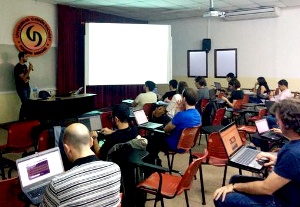
\includegraphics[width=6cm]{../../media/img/CFc8POiWYAEcPAV-small.jpg}
	\end{center}
\fi

\chapter*{Público Alvo}
\addcontentsline{toc}{chapter}{Público Alvo}

O público esperado é composto de estudantes e pesquisadores de universidades e empresas que utilizam ou tem interesse em utilizar Python em suas atividades. Espera-se um número máximo de 200 pessoas para o evento.

\begin{center}
\begin{tabular}{l c}
\bfseries{Público} & \bfseries{Esperado} \\\toprule
Professores/Pesquisadores & 50\\
Professores de & \multirow{2}{*}{20}\\
Educação básica & \\
Alunos de Pós-Graduação & 30\\
Alunos de Graduação & 60\\
Profissionais & 40\\
Outros (discriminar) & 0\\\bottomrule
\end{tabular}
\end{center}

%\ifprint
%\else
%	\begin{center}
%		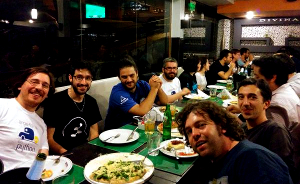
\includegraphics[width=6cm]{../../media/img/CFlOZY5WYAETG6-small.jpg}
%	\end{center}
%\fi

\chapter*{Cronograma Previsto}
\addcontentsline{toc}{chapter}{Cronograma Previsto}

As datas importantes do evento são listadas a seguir:
\begin{itemize}
\item 8 de Abril de 2016: Prazo final para submissão de palestras, pôsteres e
tutoriais.
\item 22 de Abril de 2016: Notificação de aceite para palestras, pôsteres e
tutoriais.
\item 16-17 de Maio de 2016: SciPy Latino-América 2016 - Tutoriais;
\item 18-20 de Maio de 2016: SciPy Latino-América 2016 - Palestras.
\end{itemize}

%\eject
\onecolumn
\chapter*{Coordenação da Conferência \\SciPy Latin America 2016}
\addcontentsline{toc}{chapter}{Coordenação}

\begin{tabular}{l}
\bfseries{Coordenador Geral}\\
Ivan Ogasawara\\
Telefone: (48) 9909\textendash 0207\\
\makeatletter email: ivan.ogasawara@gmail.com\makeatother \\
\\
\bfseries{Subcoordenador Geral}\\
Letícia Portella\\
\makeatletter email: leportella@gmail.com \makeatother \\
\\
Tomas Aliaga\\
\makeatletter email: taliaga@gmail.com \makeatother \\
\\
\bfseries{Coordenador Acadêmico}\\
Antonio Fernando Härter Fetter Filho\\
\makeatletter email: antonio.fetter@ufsc.br \makeatother \\
\\
\bfseries{Coordenador Científico}\\
Melissa Weber Mendonça\\
\makeatletter email: melissawm@gmail.com \makeatother \\
\\
\bfseries{Conselheiro}\\
Raniere Gaia Costa da Silva\\
Telefone: (19) 9 8819\textendash 6817\\
\makeatletter email: raniere@rgaiacs.com \makeatother \\
\end{tabular}

\section*{Outros membros}

\begin{itemize}
\item Antonio Kanaan
\item Filipe Pires Alvarenga Fernandes
\item João Felipe Nicolaci Pimentel
\item Mário Sérgio Oliveira de Queiroz
\item Matheus Braun Magrin
\end{itemize}

\section*{Embaixadores SciPy Latin America}

\begin{itemize}
\item Celia Cintas (Argentina)
\item Horacio Andres Vargas Guzmán (Bolivia)
\item Elizabeth Ramirez (Colombia)
\item Jeudy Blanco Vega (Costa Rica)
\item Olemis Lang (Cuba)
\item Sebastian Oliva (Guatemala)
\item Alex Dzul (México)
\end{itemize}

\end{document}
